%iffalse
\let\negmedspace\undefined
\let\negthickspace\undefined
\documentclass[journal,12pt,onecolumn]{IEEEtran}
\usepackage[version=4]{mhchem}
\usepackage{chemformula} % for \ch if needed
\usepackage{chemfig}
\usepackage{chemmacros}
\chemsetup{modules = reactions} % Enables reaction arrows

\usepackage{fancyhdr}
\usepackage{geometry}
\usepackage{lastpage}
\usepackage{cite}
\usepackage{amsmath,amssymb,amsfonts,amsthm}
\usepackage{enumitem,multicol}
\usepackage{algorithmic}
\usepackage{graphicx}
\usepackage{textcomp}
\usepackage{xcolor}
\usepackage{txfonts}
\usepackage{listings}
\usepackage{enumitem}
\usepackage{mathtools}
\usepackage{gensymb}
\usepackage{comment}
\usepackage[breaklinks=true]{hyperref}
\usepackage{tkz-euclide} 
\usepackage{listings}
\usepackage{gvv}                                        
%\def\inputGnumericTable{}                                 
\usepackage[utf8]{inputenc}                                
\usepackage{color}                                            
\usepackage{array}                                            
\usepackage{longtable}                                       
\usepackage{calc}                                             
\usepackage{multirow}                                         
\usepackage{hhline}                                           
\usepackage{ifthen}                                           
\usepackage{lscape}
\usepackage{tabularx}
\usepackage{array}
\usepackage{float}

\newtheorem{theorem}{Theorem}[section]
\newtheorem{problem}{Problem}
\newtheorem{proposition}{Proposition}[section]
\newtheorem{lemma}{Lemma}[section]
\newtheorem{corollary}[theorem]{Corollary}
\newtheorem{example}{Example}[section]
\newtheorem{definition}[problem]{Definition}
\newcommand{\BEQA}{\begin{eqnarray}}
\newcommand{\EEQA}{\end{eqnarray}}
\newcommand{\define}{\stackrel{\triangle}{=}}
\theoremstyle{remark}

\geometry{margin=1 in}

% Marks the beginning of the document

\title{\huge {GATE-2023-NM}}
\author{ai25btech11008- Chiruvella Harshith Sharan}
\date{}

\begin{document}

\maketitle

% Reduce spacing between items
\setlength{\parindent}{0pt}
\setlength{\parskip}{0.5cm}

\section*{Q.1 -- Q.10}

\begin{enumerate}
%------------------- Q1 -------------------%
%------------------- Q1 -------------------%
\item ``You are delaying the completion of the task. Send \_\_\_\_\_ contributions at the earliest.'' \hfill{\brak{\text{GATE NM 2023}}}

\begin{enumerate}[label=\Alph*.]
\begin{multicols}{4}
\item you are
\item your
\item you’re
\item yore
\end{multicols}
\end{enumerate}

%------------------- Q2 -------------------%
\item References : \_\_\_\_\_ : : Guidelines : Implement (By word meaning) \hfill{\brak{\text{GATE NM 2023}}}

\begin{enumerate}[label=\Alph*.]
\begin{multicols}{4}
\item Sight
\item Site
\item Cite
\item Plagiarise
\end{multicols}
\end{enumerate}

%------------------- Q3 -------------------%
\item In the given figure, PQRS is a parallelogram with $PS = 7$ cm, $PT = 4$ cm and $PV = 5$ cm.  
What is the length of $RS$ in cm? (The diagram is representative.) \hfill{\brak{\text{GATE NM 2023}}}

\begin{figure}[H]
    \centering
    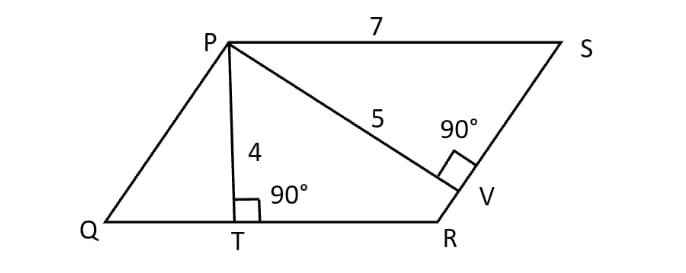
\includegraphics[scale=0.5]{figs/q3.jpg}
    \caption{}
    \label{fig:figure1}
\end{figure}

\begin{enumerate}[label=\Alph*.]
\begin{multicols}{4}
\item $20/7$
\item $28/5$
\item $9/2$
\item $35/4$
\end{multicols}
\end{enumerate}

%------------------- Q4 -------------------%
\item In 2022, June Huh was awarded the Fields medal, which is the highest prize in Mathematics.  
When he was younger, he was also a poet. He did not win any medals in the International Mathematics Olympiads.  
He dropped out of college.  

Based only on the above information, which one of the following statements can be logically inferred with certainty?\hfill{\brak{\text{GATE NM 2023}}}

\begin{enumerate}[label=\Alph*.]
\item Every Fields medalist has won a medal in an International Mathematics Olympiad.
\item Everyone who has dropped out of college has won the Fields medal.
\item All Fields medalists are part-time poets.
\item Some Fields medalists have dropped out of college.
\end{enumerate}

%------------------- Q5 -------------------%
\item A line of symmetry is defined as a line that divides a figure into two parts in a way such that each part is a mirror image of the other part about that line.  

The given figure consists of 16 unit squares arranged as shown. In addition to the three black squares, what is the minimum number of squares that must be coloured black, such that both $PQ$ and $MN$ form lines of symmetry? (The figure is representative)\hfill{\brak{\text{GATE NM 2023}}}

\begin{figure}[H]
    \centering
    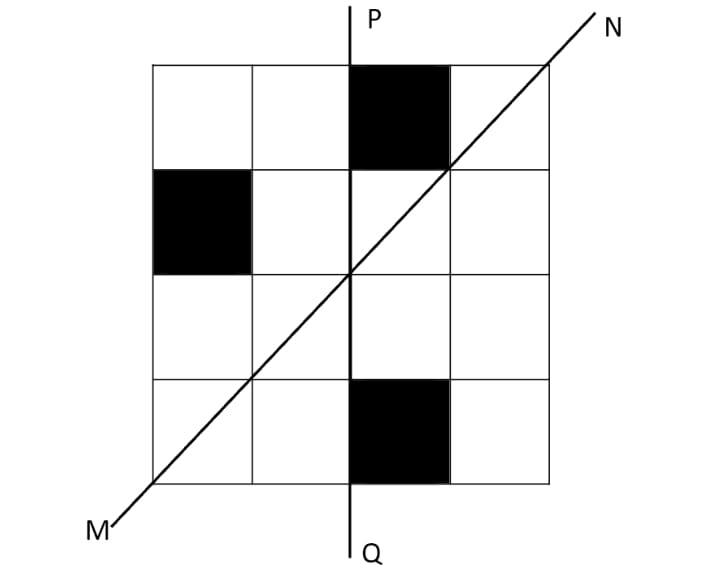
\includegraphics[scale=0.35]{figs/q5.jpg}
    \caption{}
    \label{fig:figure1}
\end{figure}

\begin{enumerate}[label=\Alph*.]
\begin{multicols}{4}
\item 3
\item 4
\item 5
\item 6
\end{multicols}
\end{enumerate}

%------------------- Q6 -------------------%
\item Human beings are one among many creatures that inhabit an imagined world.  
In this imagined world, some creatures are cruel.  
If in this imagined world, it is given that the statement ``Some human beings are not cruel creatures'' is FALSE, then which of the following set of statements can be logically inferred with certainty?  

(i) All human beings are cruel creatures.  
(ii) Some human beings are cruel creatures.  
(iii) Some creatures that are cruel are human beings.  
(iv) No human beings are cruel creatures.  \hfill{\brak{\text{GATE NM 2023}}}

\begin{enumerate}[label=\Alph*.]
\begin{multicols}{4}
\item only (i)
\item only (iii) and (iv)
\item only (i) and (ii)
\item (i), (ii) and (iii)
\end{multicols}
\end{enumerate}

%------------------- Q7 -------------------%
\item To construct a wall, sand and cement are mixed in the ratio of 3:1.  
The cost of sand and that of cement are in the ratio of 1:2.  
If the total cost of sand and cement to construct the wall is 1000 rupees, then what is the cost (in rupees) of cement used?\hfill{\brak{\text{GATE NM 2023}}}

\begin{enumerate}[label=\Alph*.]
\begin{multicols}{4}
\item 400
\item 600
\item 800
\item 200
\end{multicols}
\end{enumerate}

%------------------- Q8 -------------------%
\item The World Bank has declared that it does not plan to offer new financing to Sri Lanka, which is battling its worst economic crisis in decades, until the country has an adequate macroeconomic policy framework in place.  

In a statement, the World Bank said Sri Lanka needed to adopt structural reforms that focus on economic stabilisation and tackle the root causes of its crisis.  
The latter has starved it of foreign exchange and led to shortages of food, fuel, and medicines.  
The bank is repurposing resources under existing loans to help alleviate shortages of essential items such as medicine, cooking gas, fertiliser, meals for children, and cash for vulnerable households.  

Based only on the above passage, which one of the following statements can be inferred with certainty?  \hfill{\brak{\text{GATE NM 2023}}}

\begin{enumerate}[label=\Alph*.]
\item According to the World Bank, the root cause of Sri Lanka’s economic crisis is that it does not have enough foreign exchange. 
\item The World Bank has stated that it will advise the Sri Lankan government about how to tackle the root causes of its economic crisis.
\item According to the World Bank, Sri Lanka does not yet have an adequate macroeconomic policy framework.
\item The World Bank has stated that it will provide Sri Lanka with additional funds for essentials such as food, fuel, and medicines.
\end{enumerate}

%------------------- Q9 -------------------%
\item The coefficient of $x^4$ in the polynomial $(x - 1)^3 (x - 2)^3$ is equal to \_\_\_\_\_.\hfill{\brak{\text{GATE NM 2023}}}

\begin{enumerate}[label=\Alph*.]
\begin{multicols}{4}
\item 33
\item $-3$
\item 30
\item 21
\end{multicols}
\end{enumerate}

%------------------- Q10 -------------------%
\item Which one of the following shapes can be used to tile (completely cover by repeating) a flat plane, extending to infinity in all directions, without leaving any empty spaces in between them?  
The copies of the shape used to tile are identical and are not allowed to overlap.\hfill{\brak{\text{GATE NM 2023}}}

\begin{enumerate}[label=\Alph*.]
\begin{multicols}{4}
\item Circle
\item Regular octagon
\item Regular pentagon
\item Rhombus
\end{multicols}
\end{enumerate}

\section*{Q.11 -- Q.35}

%------------------- Q11 -------------------%
\item The velocity profile in a laminar boundary layer is $u/U = y/\delta$ where $u$ is the velocity at a distance $y$ from the wall, $U$ is the free stream velocity, and $\delta$ is the boundary layer thickness.  
The ratio of displacement thickness $(\delta^*)$ to momentum thickness $(\theta)$ is \_\_\_\_\_.\hfill{\brak{\text{GATE NM 2023}}}

\begin{enumerate}[label=\Alph*.]
\begin{multicols}{4}
\item 2.0
\item 1.5
\item 1.33
\item 1.25
\end{multicols}
\end{enumerate}

%------------------- Q12 -------------------%
\item A circular cylinder of radius $R$ is floating in water with its axis vertical. The depth of immersion of the cylinder is $R/2$.  
The density ratio of cylinder to water is \_\_\_\_\_.\hfill{\brak{\text{GATE NM 2023}}}

\begin{enumerate}[label=\Alph*.]
\begin{multicols}{4}
\item 0.25
\item 0.5
\item 0.75
\item 1.0
\end{multicols}
\end{enumerate}

%------------------- Q13 -------------------%
\item The profile of a camber line is defined by $y(x) = 2x - x^2$ where $x$ and $y$ are non-dimensional coordinates.  
The slope $\frac{dy}{dx}$ at $x = 0.5$ is \_\_\_\_\_.\hfill{\brak{\text{GATE NM 2023}}}

\begin{enumerate}[label=\Alph*.]
\begin{multicols}{4}
\item 0
\item 1
\item 2
\item 3
\end{multicols}
\end{enumerate}

%------------------- Q14 -------------------%
\item A floating body will be in stable equilibrium when\hfill{\brak{\text{GATE NM 2023}}}

\begin{figure}[H]
    \centering
    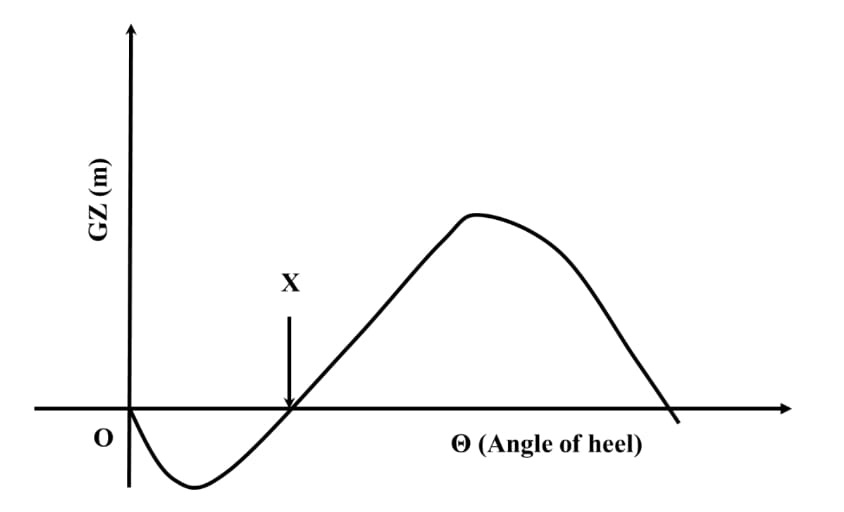
\includegraphics[scale=0.3]{figs/q14.jpg}
    \caption{}
    \label{fig:figure1}
\end{figure}

\begin{enumerate}[label=\Alph*.]
\item metacentric height is zero 
\item metacentric height is positive 
\item metacentric height is negative 
\item metacentre coincides with centre of buoyancy
\end{enumerate}

%------------------- Q15 -------------------%
\item The principal dimensions of a ship are: length $= 100$ m, breadth $= 15$ m, depth $= 10$ m, and draft $= 5$ m.  
The block coefficient is \_\_\_\_\_.\hfill{\brak{\text{GATE NM 2023}}}

\begin{enumerate}[label=\Alph*.]
\begin{multicols}{4}
\item 0.50
\item 0.67
\item 0.75
\item 1.00
\end{multicols}
\end{enumerate}

%------------------- Q16 -------------------%
\item In turbulent flow through a smooth circular pipe, the friction factor $f$ varies with Reynolds number $Re$ approximately as \_\_\_\_\_.\hfill{\brak{\text{GATE NM 2023}}}

\begin{figure}[H]
    \centering
    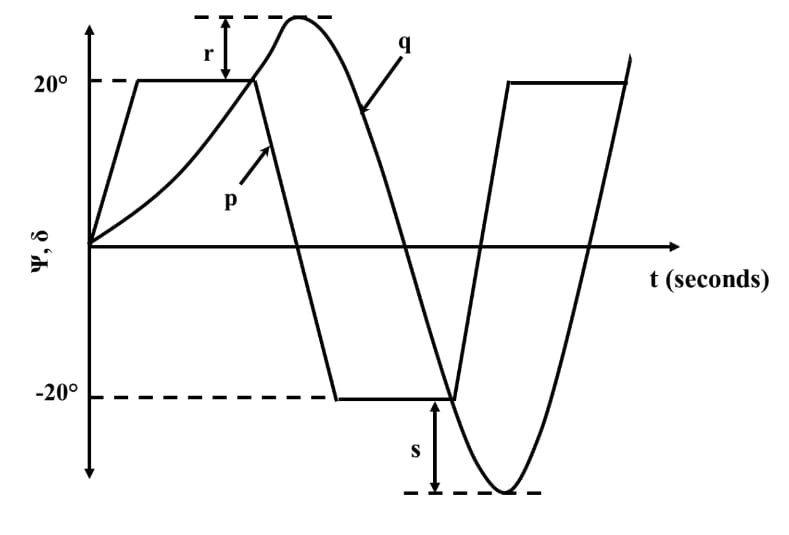
\includegraphics[scale=0.3]{figs/q16.jpg}
    \caption{}
    \label{fig:figure1}
\end{figure}

\begin{enumerate}[label=\Alph*.]
\begin{multicols}{4}
\item $f \sim 1/Re$
\item $f \sim 1/Re^{0.25}$
\item $f \sim 1/Re^{0.33}$
\item $f \sim 1/\sqrt{Re}$
\end{multicols}
\end{enumerate}

%------------------- Q17 -------------------%
\item For a hydrofoil of chord length $c$, moving with speed $V$ in water of density $\rho$, the lift per unit span is given by\hfill{\brak{\text{GATE NM 2023}}}

\begin{enumerate}[label=\Alph*.]
\begin{multicols}{4}
\item $\rho V^2 c$
\item $\frac{1}{2} \rho V^2 c$
\item $\frac{1}{2} \rho V^2 c C_L$
\item $\rho V^2 c C_D$
\end{multicols}
\end{enumerate}

%------------------- Q18 -------------------%
\item A wave of length $200$ m is propagating in deep water.  
The approximate wave celerity is \_\_\_\_\_.\hfill{\brak{\text{GATE NM 2023}}}

\begin{enumerate}[label=\Alph*.]
\begin{multicols}{4}
\item 10 m/s
\item 15 m/s
\item 20 m/s
\item 25 m/s
\end{multicols}
\end{enumerate}

%------------------- Q19 -------------------%
\item A marine propeller operates at an advance coefficient $J = 0.8$, thrust coefficient $K_T = 0.1$, and torque coefficient $K_Q = 0.02$.  
The propeller efficiency is \_\_\_\_\_.\hfill{\brak{\text{GATE NM 2023}}}

\begin{enumerate}[label=\Alph*.]
\begin{multicols}{4}
\item 0.5
\item 0.6
\item 0.7
\item 0.8
\end{multicols}
\end{enumerate}

%------------------- Q20 -------------------%
\item The natural period of rolling of a ship depends primarily on\hfill{\brak{\text{GATE NM 2023}}}

\begin{enumerate}[label=\Alph*.]
\begin{multicols}{4}
\item breadth of ship
\item length of ship
\item draft of ship
\item speed of ship
\end{multicols}
\end{enumerate}

%------------------- Q21 -------------------%
\item A slender body moving slowly in water experiences resistance mainly due to\hfill{\brak{\text{GATE NM 2023}}}

\begin{enumerate}[label=\Alph*.]
\begin{multicols}{4}
\item form drag
\item wave making drag
\item skin friction drag
\item induced drag
\end{multicols}
\end{enumerate}

%------------------- Q22 -------------------%
\item The Froude number is defined as the ratio of\hfill{\brak{\text{GATE NM 2023}}}

\begin{enumerate}[label=\Alph*.]
\item inertia force to viscous force 
\item inertia force to gravitational force
\item inertia force to elastic force 
\item inertia force to elastic force 
\end{enumerate}

%------------------- Q23 -------------------%
\item A rectangular barge is $60$ m long and $20$ m wide.  
Its displacement is $12,000$ tonnes.  
The draft of the barge is \_\_\_\_\_.\hfill{\brak{\text{GATE NM 2023}}}

\begin{figure}[H]
    \centering
    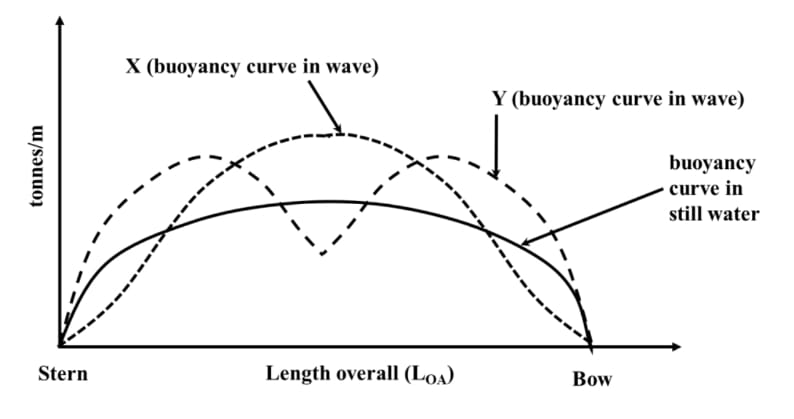
\includegraphics[scale=0.4]{figs/q23.jpg}
    \caption{}
    \label{fig:figure1}
\end{figure}

\begin{enumerate}[label=\Alph*.]
\begin{multicols}{4}
\item 5 m
\item 6 m
\item 8 m
\item 10 m
\end{multicols}
\end{enumerate}

%------------------- Q24 -------------------%
\item The restoring moment of a ship at small angles of heel is proportional to\hfill{\brak{\text{GATE NM 2023}}}

\begin{enumerate}[label=\Alph*.]
\item displacement only 
\item metacentric height only 
\item product of displacement and metacentric height
\item square of displacement
\end{enumerate}

%------------------- Q25 -------------------%
\item The metacentric height of a ship decreases when\hfill{\brak{\text{GATE NM 2023}}}

\begin{enumerate}[label=\Alph*.]
\item centre of buoyancy rises
\item metacentre rises
\item centre of gravity rises 
\item centre of gravity lowers
\end{enumerate}

%------------------- Q26 -------------------%
\item For a marine diesel engine, the mean effective pressure is $1$ MPa and displacement volume per cylinder is $1$ m$^3$.  
The indicated power per cylinder at $100$ rpm is \_\_\_\_\_.\hfill{\brak{\text{GATE NM 2023}}}

\begin{enumerate}[label=\Alph*.]
\begin{multicols}{4}
\item 1 MW
\item 1.5 MW
\item 2 MW
\item 3 MW
\end{multicols}
\end{enumerate}

%------------------- Q27 -------------------%
\item The efficiency of a diesel cycle increases if\hfill{\brak{\text{GATE NM 2023}}}

\begin{enumerate}[label=\Alph*.]
\item compression ratio increases
\item cut-off ratio increases
\item heat addition decreases
\item mean effective pressure decreases
\end{enumerate}

%------------------- Q28 -------------------%
\item The stoichiometric air-fuel ratio for diesel engines is approximately\hfill{\brak{\text{GATE NM 2023}}}

\begin{enumerate}[label=\Alph*.]
\begin{multicols}{4}
\item 5:1
\item 10:1
\item 15:1
\item 20:1
\end{multicols}
\end{enumerate}

%------------------- Q29 -------------------%
\item The stress-strain curve of mild steel under uniaxial tension shows a distinct\hfill{\brak{\text{GATE NM 2023}}}

\begin{enumerate}[label=\Alph*.]
\begin{multicols}{2}
\item elastic limit
\item yield point
\item ultimate stress point
\item fracture point
\end{multicols}
\end{enumerate}

%------------------- Q30 -------------------%
\item A thin cylindrical shell of diameter $D$ and thickness $t$ subjected to internal pressure $p$ has hoop stress\hfill{\brak{\text{GATE NM 2023}}}

\begin{enumerate}[label=\Alph*.]
\begin{multicols}{4}
\item $\frac{pD}{2t}$
\item $\frac{pD}{4t}$
\item $\frac{pD}{t}$
\item $\frac{pD}{8t}$
\end{multicols}
\end{enumerate}

%------------------- Q31 -------------------%
\item The slenderness ratio of a column is defined as\hfill{\brak{\text{GATE NM 2023}}}

\begin{enumerate}[label=\Alph*.]
\begin{multicols}{4}
\item $\frac{L}{k}$
\item $\frac{k}{L}$
\item $\frac{A}{I}$
\item $\frac{I}{A}$
\end{multicols}
\end{enumerate}

%------------------- Q32 -------------------%
\item The critical speed of a shaft is the speed at which\hfill{\brak{\text{GATE NM 2023}}}

\begin{enumerate}[label=\Alph*.]
\begin{multicols}{2}
\item the shaft bends indefinitely
\item resonance occurs
\item torque is maximum
\item power transmitted is maximum
\end{multicols}
\end{enumerate}

%------------------- Q33 -------------------%
\item The S-N curve is used in the context of\hfill{\brak{\text{GATE NM 2023}}}

\begin{enumerate}[label=\Alph*.]
\begin{multicols}{4}
\item creep
\item fatigue
\item fracture
\item impact
\end{multicols}
\end{enumerate}

%------------------- Q34 -------------------%
\item The efficiency of a riveted joint is defined as the ratio of\hfill{\brak{\text{GATE NM 2023}}}

\begin{enumerate}[label=\Alph*.]
\item strength of rivet to strength of plate 
\item strength of joint to strength of solid plate 
\item strength of plate to strength of rivet 
\item strength of rivet to strength of joint
\end{enumerate}

%------------------- Q35 -------------------%
\item The principal planes are the planes on which\hfill{\brak{\text{GATE NM 2023}}}

\begin{enumerate}[label=\Alph*.]
\begin{multicols}{2}
\item shear stress is maximum
\item shear stress is zero
\item normal stress is zero
\item normal stress is maximum
\end{multicols}
\end{enumerate}

\section*{Q.36 -- Q.65}

%------------------- Q36 -------------------%
\item The centroid of a right-angled triangle of base $b$ and height $h$, measured from the right angle, is located at\hfill{\brak{\text{GATE NM 2023}}}

\begin{enumerate}[label=\Alph*.]
\begin{multicols}{4}
\item $(b/3, h/3)$
\item $(2b/3, 2h/3)$
\item $(b/2, h/2)$
\item $(b/4, h/4)$
\end{multicols}
\end{enumerate}

%------------------- Q37 -------------------%
\item A simply supported beam of length $L$ carries a uniformly distributed load $w$ per unit length.  
The maximum bending moment is\hfill{\brak{\text{GATE NM 2023}}}

\begin{enumerate}[label=\Alph*.]
\begin{multicols}{4}
\item $wL/4$
\item $wL^2/8$
\item $wL^2/12$
\item $wL^2/16$
\end{multicols}
\end{enumerate}

%------------------- Q38 -------------------%
\item A cantilever beam of length $L$ carries a concentrated load $P$ at the free end.  
The deflection at the free end is $\frac{PL^3}{3EI}$.  
If the beam length is doubled, keeping $P$, $E$, and $I$ same, the deflection will increase by a factor of\hfill{\brak{\text{GATE NM 2023}}}

\begin{figure}[H]
    \centering
    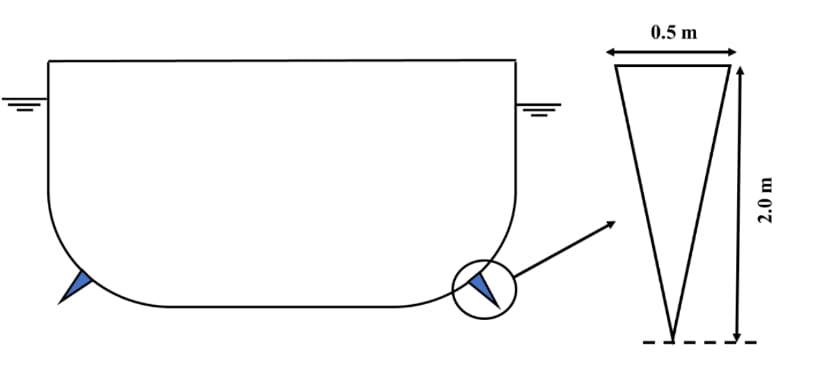
\includegraphics[scale=0.35]{figs/q38.jpg}
    \caption{}
    \label{fig:figure1}
\end{figure}

\begin{enumerate}[label=\Alph*.]
\begin{multicols}{4}
\item 2
\item 4
\item 6
\item 8
\end{multicols}
\end{enumerate}

%------------------- Q39 -------------------%
\item The shear force at the free end of a cantilever beam carrying a point load at the free end is\hfill{\brak{\text{GATE NM 2023}}}

\begin{enumerate}[label=\Alph*.]
\begin{multicols}{2}
\item zero
\item equal to the load
\item maximum at fixed end
\item equal to bending moment
\end{multicols}
\end{enumerate}

%------------------- Q40 -------------------%
\item A circular shaft subjected to torsion experiences maximum shear stress at\hfill{\brak{\text{GATE NM 2023}}}

\begin{enumerate}[label=\Alph*.]
\begin{multicols}{4}
\item centre
\item surface
\item middle radius
\item along axis
\end{multicols}
\end{enumerate}

%------------------- Q41 -------------------%
\item Euler’s buckling load for a column with both ends hinged is $P_{cr} = \frac{\pi^2 EI}{L^2}$.  
If one end is fixed and the other free, the buckling load is\hfill{\brak{\text{GATE NM 2023}}}

\begin{enumerate}[label=\Alph*.]
\begin{multicols}{4}
\item $\frac{\pi^2 EI}{L^2}$
\item $\frac{\pi^2 EI}{4L^2}$
\item $\frac{\pi^2 EI}{2L^2}$
\item $\frac{\pi^2 EI}{L^2/4}$
\end{multicols}
\end{enumerate}

%------------------- Q42 -------------------%
\item For an incompressible fluid, the continuity equation is\hfill{\brak{\text{GATE NM 2023}}}

\begin{enumerate}[label=\Alph*.]
\begin{multicols}{4}
\item $\nabla \cdot \vec{V} = 0$
\item $\nabla \times \vec{V} = 0$
\item $\nabla \cdot \vec{V} = \rho$
\item $\nabla \times \vec{V} = \rho$
\end{multicols}
\end{enumerate}

%------------------- Q43 -------------------%
\item Bernoulli’s equation represents conservation of\hfill{\brak{\text{GATE NM 2023}}}

\begin{enumerate}[label=\Alph*.]
\begin{multicols}{4}
\item mass
\item energy
\item momentum
\item vorticity
\end{multicols}
\end{enumerate}

%------------------- Q44 -------------------%
\item Kelvin’s circulation theorem applies to\hfill{\brak{\text{GATE NM 2023}}}

\begin{enumerate}[label=\Alph*.]
\begin{multicols}{2}
\item viscous flows
\item irrotational flows
\item inviscid barotropic flows
\item compressible flows
\end{multicols}
\end{enumerate}

%------------------- Q45 -------------------%
\item The Prandtl number is defined as the ratio of\hfill{\brak{\text{GATE NM 2023}}}

\begin{enumerate}[label=\Alph*.]
\item momentum diffusivity to thermal diffusivity
\item thermal diffusivity to momentum diffusivity 
\item viscosity to conductivity 
\item Reynolds number to Nusselt number
\end{enumerate}

%------------------- Q46 -------------------%
\item The Mach number is defined as the ratio of\hfill{\brak{\text{GATE NM 2023}}}

\begin{figure}[H]
    \centering
    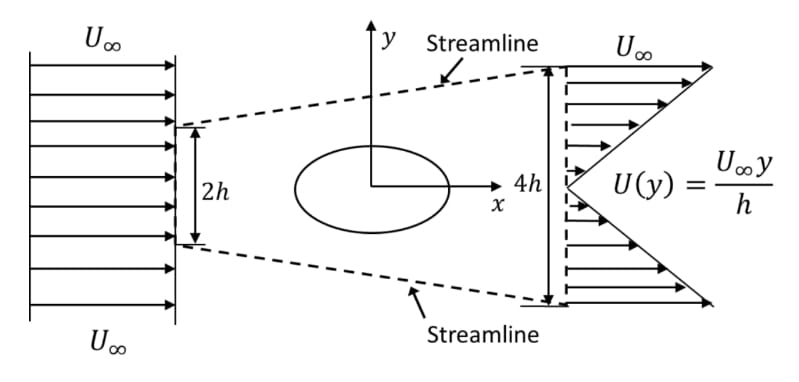
\includegraphics[scale=0.4]{figs/q46.jpg}
    \caption{}
    \label{fig:figure1}
\end{figure}

\begin{enumerate}[label=\Alph*.]
\begin{multicols}{2}
\item flow velocity to local speed of sound
\item pressure to density
\item inertia to compressibility
\item velocity head to pressure head
\end{multicols}
\end{enumerate}

%------------------- Q47 -------------------%
\item The lift coefficient $C_L$ for a thin airfoil at small angle of attack $\alpha$ (in radians) is approximately\hfill{\brak{\text{GATE NM 2023}}}

\begin{enumerate}[label=\Alph*.]
\begin{multicols}{4}
\item $2\pi \alpha$
\item $\pi \alpha$
\item $4\pi \alpha$
\item $\alpha$
\end{multicols}
\end{enumerate}

%------------------- Q48 -------------------%
\item For a propeller, the thrust $T$ is given by $T = \rho n^2 D^4 K_T$, where $n$ is revolutions per second and $D$ is diameter.  
The unit of $K_T$ is\hfill{\brak{\text{GATE NM 2023}}}

\begin{enumerate}[label=\Alph*.]
\begin{multicols}{4}
\item dimensionless
\item length
\item time
\item force
\end{multicols}
\end{enumerate}

%------------------- Q49 -------------------%
\item The efficiency of a propeller is maximum when the slip ratio is\hfill{\brak{\text{GATE NM 2023}}}

\begin{enumerate}[label=\Alph*.]
\begin{multicols}{4}
\item zero
\item small positive
\item large positive
\item negative
\end{multicols}
\end{enumerate}

%------------------- Q50 -------------------%
\item A ship of length $L$ moving with speed $V$ in deep water will have wave-making resistance that primarily depends on\hfill{\brak{\text{GATE NM 2023}}}

\begin{enumerate}[label=\Alph*.]
\begin{multicols}{4}
\item Froude number
\item Reynolds number
\item Mach number
\item Weber number
\end{multicols}
\end{enumerate}

%------------------- Q51 -------------------%
\item In a four-stroke diesel engine, one power stroke occurs in\hfill{\brak{\text{GATE NM 2023}}}

\begin{enumerate}[label=\Alph*.]
\begin{multicols}{2}
\item 180° crank rotation
\item 360° crank rotation
\item 540° crank rotation
\item 720° crank rotation
\end{multicols}
\end{enumerate}

%------------------- Q52 -------------------%
\item The brake power of an IC engine is measured using\hfill{\brak{\text{GATE NM 2023}}}

\begin{enumerate}[label=\Alph*.]
\begin{multicols}{4}
\item calorimeter
\item manometer
\item dynamometer
\item orifice meter
\end{multicols}
\end{enumerate}

%------------------- Q53 -------------------%
\item For an ideal Otto cycle, the efficiency depends only on\hfill{\brak{\text{GATE NM 2023}}}

\begin{enumerate}[label=\Alph*.]
\begin{multicols}{4}
\item compression ratio
\item expansion ratio
\item cut-off ratio
\item clearance volume
\end{multicols}
\end{enumerate}

%------------------- Q54 -------------------%
\item The brake thermal efficiency of an IC engine is the ratio of\hfill{\brak{\text{GATE NM 2023}}}

\begin{enumerate}[label=\Alph*.]
\begin{multicols}{2}
\item brake power to heat supplied
\item brake power to indicated power
\item indicated power to brake power
\item indicated power to heat supplied
\end{multicols}
\end{enumerate}

%------------------- Q55 -------------------%
\item The volumetric efficiency of a compressor is defined as the ratio of\hfill{\brak{\text{GATE NM 2023}}}

\begin{enumerate}[label=\Alph*.]
\begin{multicols}{2}
\item swept volume to clearance volume
\item actual intake to swept volume
\item actual intake to theoretical intake
\item theoretical intake to swept volume
\end{multicols}
\end{enumerate}

%------------------- Q56 -------------------%
\item The thermal efficiency of a Rankine cycle increases with\hfill{\brak{\text{GATE NM 2023}}}

\begin{enumerate}[label=\Alph*.]
\begin{multicols}{2}
\item increasing condenser pressure
\item decreasing boiler pressure
\item superheating of steam
\item decreasing turbine inlet temperature
\end{multicols}
\end{enumerate}

%------------------- Q57 -------------------%
\item The coefficient of performance (COP) of a refrigerator is defined as\hfill{\brak{\text{GATE NM 2023}}}

\begin{figure}[H]
    \centering
    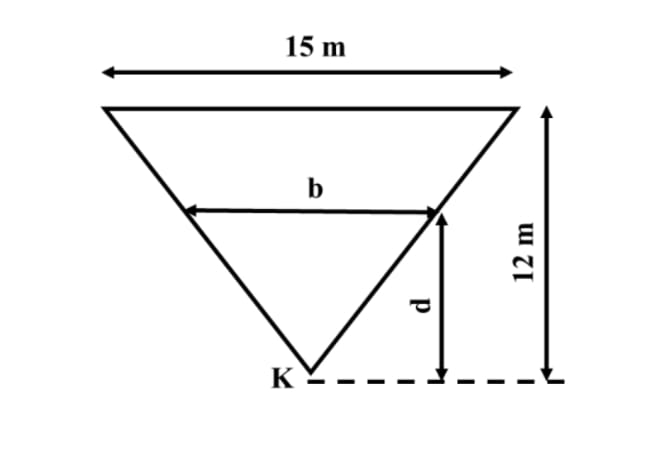
\includegraphics[scale=0.35]{figs/q57.jpg}
    \caption{}
    \label{fig:figure1}
\end{figure}

\begin{enumerate}[label=\Alph*.]
\item heat absorbed in condenser / work input
\item heat absorbed in evaporator / work input
\item work input / heat absorbed in condenser 
\item work input / heat absorbed in evaporator
\end{enumerate}

%------------------- Q58 -------------------%
\item In welding, lack of fusion is a type of\hfill{\brak{\text{GATE NM 2023}}}

\begin{enumerate}[label=\Alph*.]
\begin{multicols}{2}
\item surface defect
\item subsurface defect
\item volumetric defect
\item dimensional defect
\end{multicols}
\end{enumerate}

%------------------- Q59 -------------------%
\item In casting, risers are used to\hfill{\brak{\text{GATE NM 2023}}}

\begin{enumerate}[label=\Alph*.]
\item provide molten metal to compensate shrinkage
\item improve surface finish
\item control solidification rate 
\item improve machinability
\end{enumerate}

%------------------- Q60 -------------------%
\item In gas welding, the commonly used fuel gas is\hfill{\brak{\text{GATE NM 2023}}}

\begin{enumerate}[label=\Alph*.]
\begin{multicols}{4}
\item methane
\item propane
\item acetylene
\item butane
\end{multicols}
\end{enumerate}

%------------------- Q61 -------------------%
\item In orthogonal cutting, the shear angle is the angle between\hfill{\brak{\text{GATE NM 2023}}}

\begin{enumerate}[label=\Alph*.]
\begin{multicols}{2}
\item shear plane and cutting velocity
\item shear plane and rake face
\item cutting edge and work surface
\item rake angle and clearance angle
\end{multicols}
\end{enumerate}

%------------------- Q62 -------------------%
\item Tool life is generally represented by the Taylor’s equation $VT^n = C$, where $n$ is typically in the range of\hfill{\brak{\text{GATE NM 2023}}}

\begin{enumerate}[label=\Alph*.]
\begin{multicols}{4}
\item 0.01–0.05
\item 0.1–0.2
\item 0.2–0.6
\item 0.7–1.0
\end{multicols}
\end{enumerate}

%------------------- Q63 -------------------%
\item Gantt charts are used for\hfill{\brak{\text{GATE NM 2023}}}

\begin{enumerate}[label=\Alph*.]
\begin{multicols}{4}
\item inventory control
\item project scheduling
\item quality control
\item material handling
\end{multicols}
\end{enumerate}

%------------------- Q64 -------------------%
\item The Economic Order Quantity (EOQ) is the order quantity that\hfill{\brak{\text{GATE NM 2023}}}

\begin{enumerate}[label=\Alph*.]
\begin{multicols}{2}
\item minimizes total cost
\item maximizes profit
\item minimizes holding cost
\item minimizes ordering cost
\end{multicols}
\end{enumerate}

%------------------- Q65 -------------------%
\item PERT is a project management technique primarily concerned with\hfill{\brak{\text{GATE NM 2023}}}

\begin{figure}[H]
    \centering
    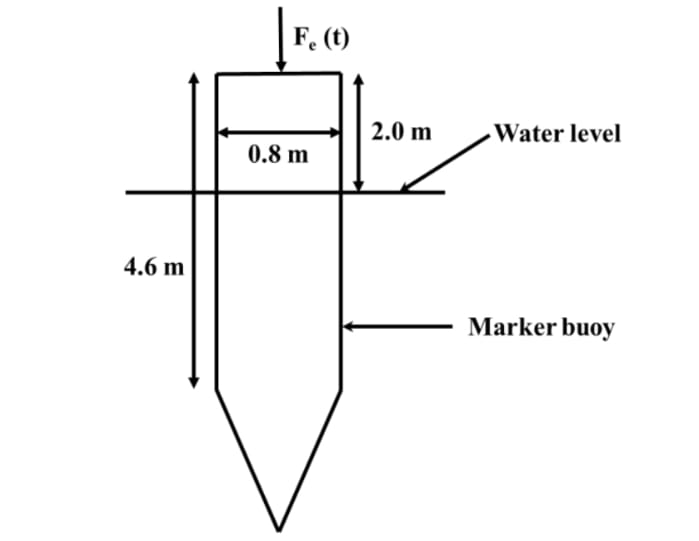
\includegraphics[scale=0.35]{figs/q65.jpg}
    \caption{}
    \label{fig:figure1}
\end{figure}

\begin{enumerate}[label=\Alph*.]
\begin{multicols}{4}
\item time
\item cost
\item resources
\item quality
\end{multicols}
\end{enumerate}


\end{enumerate}

\begin{center}
\section*{END OF QUESTION PAPER}
\end{center}


\end{document}